\documentclass[stu,biblatex,floatsintext,draftall]{apa7}

\usepackage{graphicx}
\graphicspath{{assets/}}

\usepackage{siunitx}

\addbibresource{refs.bib}

\title{Investigating the Effect of Chain Length on Acceleration}
\author{Adam Zhang}
\affiliation{Academies of Loudoun}
\course{AP Physics C: Mech, Block 2}
\professor{Matthew Hilsdorf}
\duedate{September 21 2023}

\begin{document}
\maketitle
\tableofcontents
\newpage

\section{Introduction}

\subsection{Purpose}
Investigate the effect of the length of a heavy chain on the rate of change of the acceleration (jerk) of the chain as it falls off a pulley.

\subsection{Hypothesis}
An increase in the length of the chain will result in an increase in the rate of change of acceleration (jerk) of the chain.

\subsection{Background}
Describe relevant background, concepts, and applicable equations, with citations.

\section{Methods}

\subsection{Materials}
The following materials are required for this experiment \parencite{Hilsdorf2023AtwoodsHeavyChainHandout}:
\begin{APAitemize}
	% TODO Add links and symbols
	\item Vernier ultra pulley (green)
	\item Vernier photogate and connection cable
	\item Vernier LabQuest
	\item Meter stick
	\item Chains of varying lengths % TODO clarify
\end{APAitemize}
The setup of the experiment is shown in Figure \ref{fig:setup}.
\begin{figure}
	\centering
	\caption{Experimental Setup}
	\label{fig:setup}
	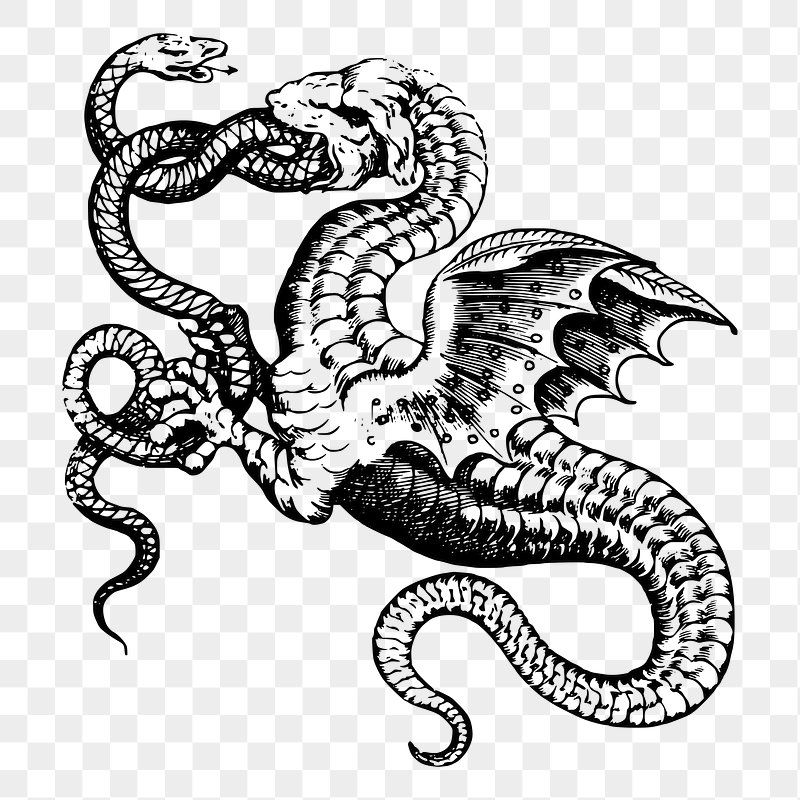
\includegraphics{dragon}
\end{figure}

\subsection{Procedures}
The following procedure was implemented during this experiment.
\begin{APAenumerate}
	\item Construct the experimental setup as shown in Figure \ref{fig:setup}.
	\item\label{pro:outer-start} Place the 60\unit{\centi\meter} chain on the pulley so that 25\unit{\centi\meter} of the chain is on the side away from the photogate.
	\item\label{pro:inner-start} Start collecting data on the LabQuest, then release the chain.
	\item\label{pro:inner-end} End the data collection after the chain has fallen.
	\item\label{pro:outer-end} Repeat steps \ref{pro:inner-start} through \ref{pro:inner-end} two more times to obtain 3 total trials for this length.
	\item Repeat steps \ref{pro:outer-start} through \ref{pro:outer-end} four more times, increasing the chain length by 10\unit{\centi\meter} every time to obtain a total of 15 trials.
\end{APAenumerate}

\section{Results}
\subsection{Data}
\begin{table}
	\centering
	\caption{Caption}
	\label{tab:data}
	\begin{tabular}{cc}
		Column 1 & Column 2 \\
		\hline
		Data 1 & Data 2
	\end{tabular}
\end{table}
\begin{figure}
	\caption{Graph}
	\label{fig:data-graph}
	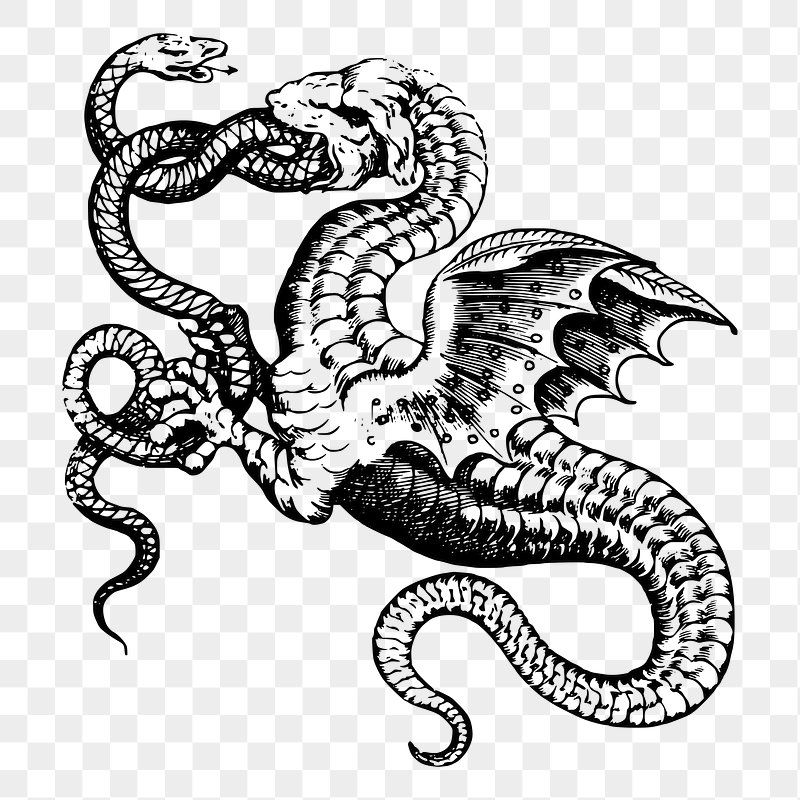
\includegraphics{dragon}
\end{figure}

\subsection{Calculations}
Insert an example calculation.  Do not write out “multiply velocity times time…”  Define your parameters, use numbers, and equations. Include the general formula, formula with numbers, and final answer with units. Show \% error calculation steps, if applicable.

\section{Discussion}

\subsection{Conclusion}
Discuss if the hypothesis was satisfied, including data/evidence from experiment. Reflect on the success/failure of the experiment (purpose accomplished or not). Make a claim, support it with evidence from the experiment, and use reasoning related to the principles discussed in the background to support it.

\subsection{Errors}
Describe errors and sources of error. Be specific. Comment on the percent error calculation (if applicable).  Include a discussion of how to minimize error in further research. 

\subsection{Extensions}
Explain how the conclusions and experiment are relevant to real-life.  Provide commentary to answer required questions. 

\printbibliography

\end{document}
